\documentclass[12pt]{article}
\usepackage{fullpage}
\usepackage{epsf}
\usepackage{epsfig}
\usepackage{amsthm}
\usepackage{amsfonts}
\usepackage{color}
\usepackage{amsmath}
\usepackage{setspace}
\usepackage{natbib}
\usepackage{hyperref}
\usepackage{algorithmic}
\usepackage[boxed]{algorithm}
\usepackage[usenames, dvipsnames]{xcolor}

\usepackage{graphicx}
\usepackage{caption}
\usepackage{subcaption}
\usepackage[normalem]{ulem}

\begin{document}


%%%%%%%%%%%%%%%%%%%%%%%%%%%%%%%%%%%%%%%%%%%%%%%%%%%%%%%%%%%%%%%%%%%%%%%%%%%%%%%%%%%%%%%%%%%%%%%%%%%%%%%%%%%


\title{\vspace{-1cm}
A shiny update to an old experiment game}
\author{
Robert B.~Gramacy\\
Department of Statistics\\
Virginia Tech\thanks{{\em Contact:} {\tt rbg@vt.edu} or Hutcheson Hall (MCO439),
250 Drillfield Drive, Blacksburg, VA 24061}}
\date{}
\maketitle


\begin{abstract}
A full appreciation of aspects of experimental design, modeling, and
decision making in applied settings takes time, in two senses. That learning
requires patience and diligence is the first, obvious, sense. The second one
is that applied work, and experimentation, often play out over long time
scales, during which theories are revised, model and inferential techniques
are improved, and knowledge is updated. Here I present a game,
borrowing liberally from one first played over forty years ago, that attempts
to synergize these aspects of learning time.   The goal is to reinforce a
cascade of topics in modern response surface methods, sequential design and
optimization, in a stimulating, competitive and realistic environment.
Interface, rules, and evaluation are described, along with a ``case study''
involving a cohort of students at Virginia Tech.

  \bigskip
  \noindent {\bf Key words:}
  response surface, computer experiment, experimental design, Bayesian optimization, input sensitivity, teaching game
\end{abstract}

%\vspace{1cm}

\doublespacing
%\onehalfspacing

\section{The setting}
\label{sec:intro}


In-class games are a common way to encourage learning---to interject some fun
and build intuition in an seemingly esoteric, or tedious technical landscape.
A good game could be fundamental to retaining students, say in introductory
statistics.  One fine example uses chocolate chip cookies to illustrate
aspects of sampling distributions \citep{lee:2007}.  The long arc of an
out-of-class game played over an entire semester is attempted rather less
frequently. However for some topics, like experimental design and response
surface optimization, that setting is quite natural: real-life applications
play out on longer temporal scales, and in an inherently dynamic landscape. In
this article I present such a game, which was played during a graduate
course I recently gave at Virginia Tech. The game is an update of one
first played over forty years ago \citep{mead:freeman:1973}.

\citeauthor{mead:freeman:1973}'s game was ahead of its time.  Today it is all
but forgotten. Although it is cited prominently in  \cite{box:draper:1987},
which is how I found it, that is one of just eight references in the
literature. Perhaps this is because, for many decades (70s-90s, say) the setup
of the game, requiring a custom computing environment with student access, was
hard to replicate.  Today, with {\sf R}/CRAN \citep{cranR} implementation and
{\tt shiny} \citep{shiny} web interfaces, barriers have come way down.
  
The original game involves {\em blackbox} evaluation of agricultural yield
as a function of six nutrient levels, borrowed from \cite{nelder:1966} and
reproduced in {\sf R} as follows.

{\singlespacing
\begin{verbatim}
yield <- function(N, P, K, Na, Ca, Mg)
{
  l1 <- 0.015 + 0.0005*N + 0.001*P + 1/((N+5)*(P+2)) + 0.001*K + 0.1/(K+2)
  l2 <- 0.001*((2 + K + 0.5*Na)/(Ca+1)) + 0.004*((Ca+1)/(2 + K + 0.5*Na))
  l3 <- 0.02/(Mg+1)
  return(1/(l1 + l2 + l3))
}
\end{verbatim}}

\noindent Although my updated game has kept this {\tt yield} form in its
inaugural run, swapping in code for a new blackbox is a trivial matter. Section
\ref{sec:discuss} discusses some potential alternatives.

The original game involved observations of {\tt yield} with additive
(Gaussian) block and plot-within-block effects.  Players could obtain noisy
{\tt yield} evaluations, with the ultimate goal of maximizing, across up to
five computer sessions (simulating crop years).  Multiple experiments could be
undertaken in a single session; however strategies could only be revised
``between years''. My updated version retains this spirit of play, but differs
on many specifics, as detailed in Section \ref{sec:game}.

Adaptations in the new game are motivated by technology, and a desire to teach
a more modern statistical toolkit.  Classical response surface methods, and
design, emphasize low degree (first- and second-order) linear modeling.  The
resulting steepest ascent and ridge analyses \citep[see,
e.g.,][]{box:draper:1987,myers:etal:2016} enjoy a high degree of analytical
tractability. Many relevant calculations can either be performed by hand, or
with a graphing calculator.  Yet such tools represent the tip of the iceberg
in modern application domains like information technology. They seem
particularly crude in situations where physical experimentation is coupled
with computer simulation experiments, a setup originating in physics and
engineering, but becoming increasingly commonplace in the other applied sciences.
Modern response surface methods borrow heavily from geostatistics and machine
learning with Gaussian processes, deep neural networks, and regression and
classification trees.  Sequential design strategies like expected improvement
\citep{jones:schonlau:welch:1998} promise a more modular approach to
(so-called Bayesian) optimization, allowing fancy models to be swapped in and out,
and a degree of human-free automation with light coding.

Exploring a diverse, state-of-the-art, toolkit benefits from sandboxing
aspects of game play, but moreover the superlative nature of the goal---of
optimizing {\tt yield}---perhaps suggests that an element of competition may
further enhance the learning arena.  Section \ref{sec:outcomes} covers player
benchmarking, timing of methodology with lecture material, and an assessment
strategy designed to encourage regular engagement and the deployment of a
wealth of tools.  Some results from a real run of the game at Virginia Tech
are provided.  Section \ref{sec:discuss} concludes with lessons learned and
ideas for future variations.  The online supplement includes a full suite of
supporting codes and other teaching materials.

\section{Game design}
\label{sec:game}

The core of game play is facilitated by an {\sf R} {\tt shiny} app, shown in
Figure \ref{f:app}, which serves as both a multi-player portal and an
interface to the back-end database of player(s) records.  An {\tt Rmarkdown}
document, {\tt yield.Rmd}, provided with the supplementary material, compiles
a full set of instructions on how to use the app, the rules of the game, and
some suggestions about strategy.  An HTML rendering of that document is
provided at \url{http://bobby.gramacy.com/teaching/rsm/yield.html}.  The
salient details follow.

\subsection{Using the {\tt shiny} app}

Since all game players use the same app, interaction begins with a ``logging
in'' phase.  In advance of opening the game, I asked each player to provide me
with their initials (2--4 characters) and a four-digit secret PIN, the
combination of which is comprises of the login token.  Logging in involves
providing ``url?token'' in the browser search bar.  In Figure \ref{f:app} the
URL points to a local {\tt shiny} server, and the token is ``rbg4036'', a
combination of my initials (I played the game too) and my office number, 403G.

\begin{figure}[ht!]
\centering
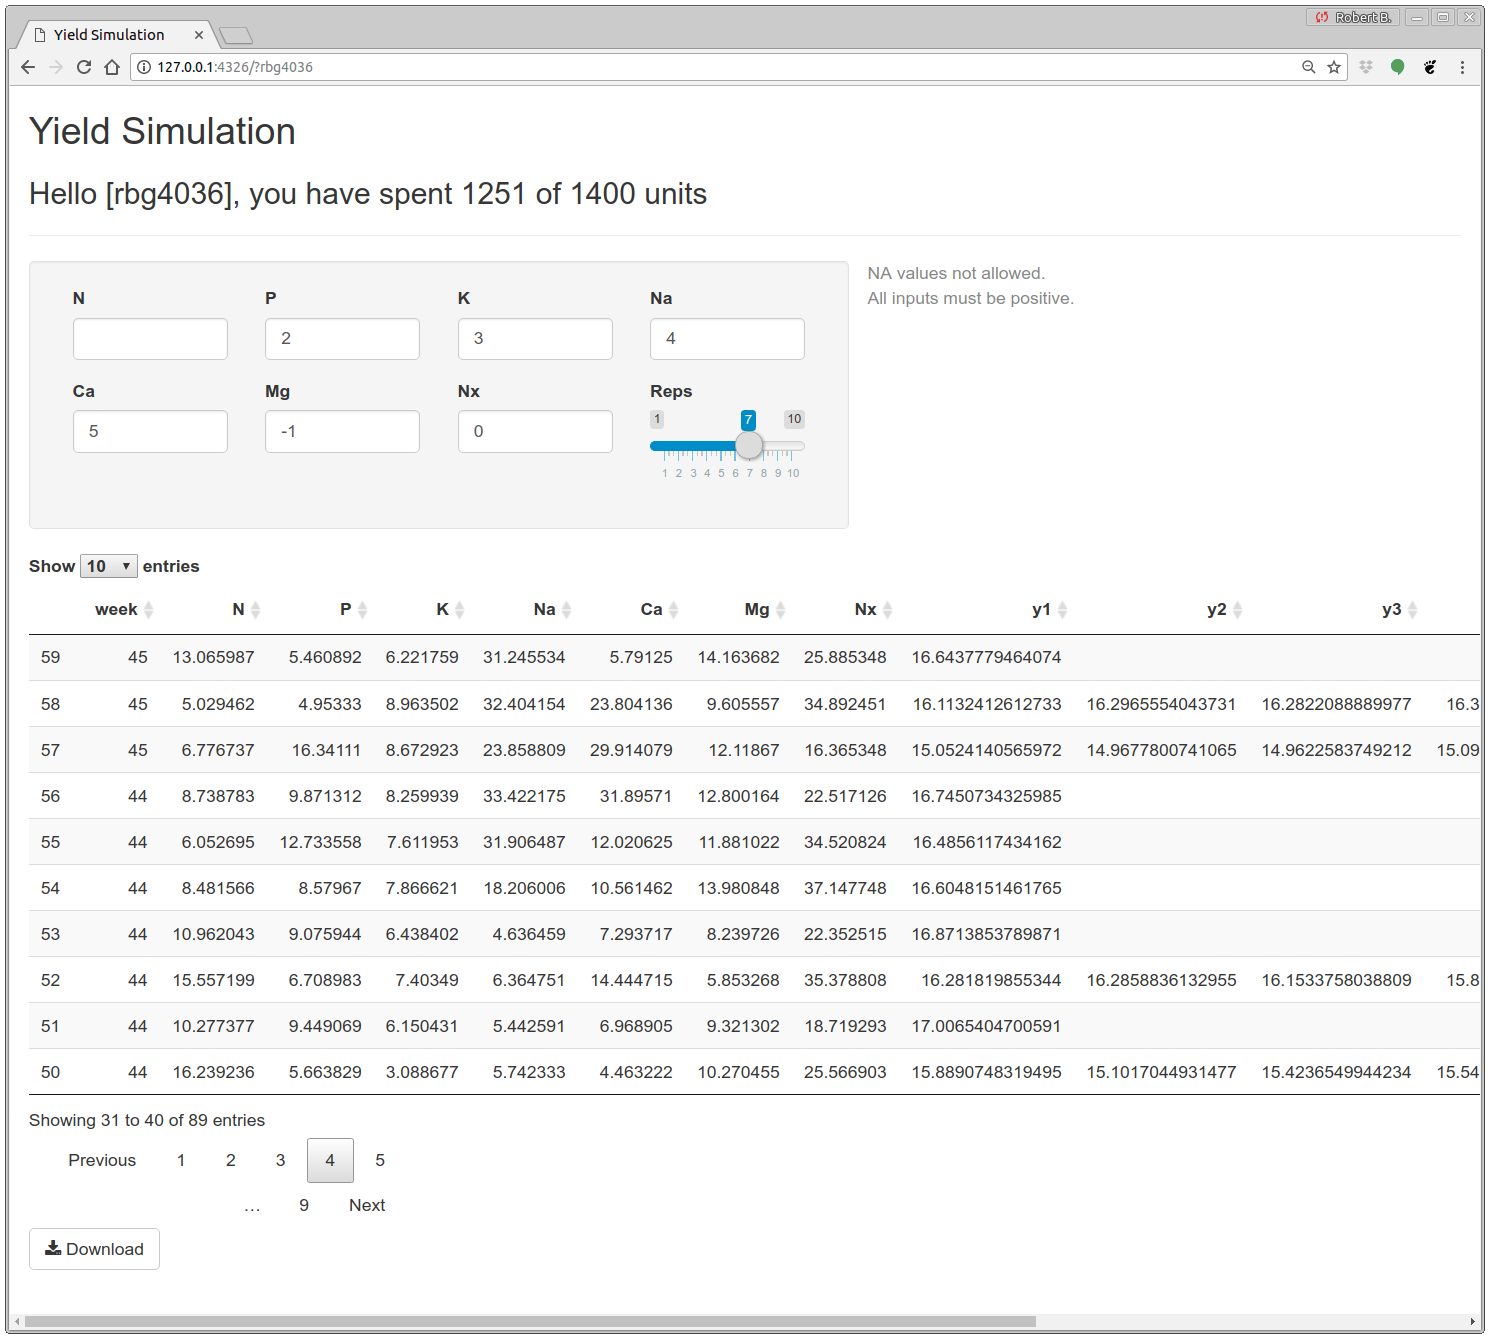
\includegraphics[scale=0.31]{app}
\caption{An interactive {\tt yield} simulation session. User {\tt rbg4036} may
inspect the run budget, perform new runs (if budget remains), browse
historical runs, or download a text file.}
\label{f:app}
\end{figure}

Once logged in, the player is presented with three blocks of game content. A
greeting block provides details on spent and total budget for experimental
runs.  How the budget works, costs of runs, etc., is discussed in detail in
Section \ref{sec:rules}.  As long as the player has not fully spent, or
over-spent, their budget, new runs may be performed, via the second block on
the page. Here, the player enters the coordinates of the next run.  Until all
fields are populated with valid (positive, non-empty) values, helpful error
messages appear on the right.  The last input, which is a slider, indicates
the number of replicates desired---again discussed in more detail
shortly. Once all entries are valid, the error messages are replaced by a
``Run'' button and a warning that there are no do-overs.

Performing a run causes the table in the final block of the page to be
updated, with the inputs and outputs of the new run appearing at the top of
the table.  All together, the table has 18 columns, recording the run week, 7
inputs, and up to ten outputs.  The primary purpose of the table is to provide
visual confirmation that the run has been successfully stored in the player's
database file. Buttons are provided to aid in browsing, however this is not
intended as the main data-access vehicle.  A ``Download'' button at the bottom
creates a text file which can be saved via browser support---usually into the
\verb|~/Downloads| directory. Empty output fields are converted to {\tt NA}s
in the downloaded file.

Under the hood, the app maintains the player database as files quite
similar to those offered for downloading.  If the app is being hosted on a
standalone node running a {\tt shiny} server, those files may be stored
locally in the app's working directory.  However, if the game is hosted in the
cloud, say on
\verb!shinyapps.io!, the database can only temporarily be stored locally,
while that instance is active. Ensuring that each of multiple running
instances share the same game database,  and guaranteeing its integrity after
an instance times out due to inactivity (which causes the local running
directory to be purged), requires that the files be stored elsewhere, in a
single persistently available location in the cloud. I hosted my game at
\url{http://gramacylab.shinyapps.io/yield}, with database files at
\url{www.dropbox.com} accessed through the {\tt rdrop2} \citep{rdrop2} API.
When a new instance is created, startup code triggers {\tt rdrop2} calls to
\verb!drop_get! files into the local working directory,\footnote{All of the
player files are downloaded as part of the instance initialization, which can
unfortunately be time consuming. However, the instance is then ready to serve
multiple players, if needed.} and subsequently \verb!drop_upload! to sync
those with new runs.

\subsection{Rules, startup and twists}
\label{sec:rules}

Many of the rules of the game are enforced by the interface.  The most
important exception is to do with players sharing data files and/or login
tokens, which is not allowed. Players are encouraged to collaborate on
strategy, and the development of relevant mathematical calculations, but they
may not share code or data.  All players start with a database containing an
identical design of seven input settings, each with five replicate responses
whose noise structure is explained momentarily.  Students were introduced to
the game in the fifth week (game week zero), and could perform their first
runs in the sixth week of a 15-week semester. Including Thanksgiving and a
final exams tallies thirteen weeks of game play.

In each week, including week zero, students accrued 100 playing units to spend
on runs, with full roll-over from previous weeks.  The cost structure for runs
favors replicates.  Obtaining a single run (i.e., the first replicate) costs
ten units.  Replicates two through four cost an additional three units each; five
through seven cost two, and eight through ten cost one each.  As long as a player's
account is in the black (i.e., positive balance), s/he can perform a new run
with as many replicates as desired.  If performing that run causes the balance
to be zero, or negative, future runs will not be allowed (the run box on the
app disappears) until the following week, after 100 new units are added.

Replication is important for two game ``twists'' designed to encourage players
to think about signal-to-noise trade-offs, and to nudge them to spend
units regularly, rather than save them all until the end of the semester.  The
first is that players are told that the variance of the additive noise on {\tt
yield} is changing weekly, following a smooth process in time, and that they
will need to provide an estimate of that variance over time for their final
report.  They are further warned that the variance may be increasing,
effectively devaluing unused units.  In fact the variance in
week $w$ followed a simple sinusoidal structure
\[
\sigma^2(w) = 0.1 + 0.05 (\cos(2\pi(w - w_s)/10)+1) \quad\quad \mbox{for starting week} \; w_s,
\]
 which peaks in the first and tenth week.  The second wrinkle is a seventh
input, {\tt Nx}, which is unrelated to the response.  Students are not told
that one of the inputs is useless, however the final writeup instructions ask
for sensitivity analyses for the inputs, including main, partial dependence,
and total effects.

\section{Timing, outcomes and evaluation}
\label{sec:outcomes}

Starting in the fifth week of the semester allows for ramp-up on
methodological training, giving students the chance to learn fundamentals like
steepest ascent and ridge analyses \citep[e.g.,][Chapters
5--6]{myers:etal:2016} before entering the game as players. Using {\sf R} code
provided in class, most students were able perform runs in the first two weeks
that improved upon {\tt yield}s from week zero. In subsequent weeks, new
methodology was introduced which students were expected to try in the game.
Details on how game play tracks course material, cookie crumbs to ``catch up''
stragglers, and windows into game progress are provided below.


\subsection{Subject progression and homeworks}

Homeworks are assigned roughly every two weeks and each one, from the third
onward, contains a problem on the game. Problem statements and solutions are
provided with the supplementary material. The third homework is the the most
prescriptive about what to do in the game.  It instructs the student to fit a
first-order model to the initial data set ($7
\times 5$ runs) and determine which of the seven main effects are useful for
describing variation in {\tt yield}. In my own solution, only the first three
are relevant, e.g., after a backwards {\tt step}-wise selection procedure with
BIC.  Then, after reducing to a first order model having only those three
components, they are asked to search for interactions.  I found one.

With best fitted model in hand, students are asked to characterize a path of
steepest ascent, and to obtain {\tt yield} responses along that path.  This
requires determining values for the remaining (in my case four) inputs. No
guidance is given here; I used a Latin hypercube sample, paired with six
settings of the three active variables a short ways along the path of steepest
ascent.  Next, students are given several options about how to proceed,
including a second-order ridge analysis, more exploration with space-filling
designs, or more steepest ascent.  In my own solution I did a bit of all
three, and the result was a second-order fit to the data that had many
relevant main effects, interactions, etc.

After the homework deadline, I released my solution so students could see what
I did, and use it to ``catch up'' with other players during subsequent weeks.
Then we transitioned to modern material involving Gaussian processes (GPs),
presented from machine learning \citep{rasmu:will:2006} and computer surrogate
modeling \citep{sant:will:notz:2003} perspectives.  Both communities
evangelize the potential for fitted GP predictive surfaces to guide searches
for global optima in blackbox functions. Machine learning researchers call
this Bayesian optimization, whereas computer modelers call it
surrogate-assisted optimization (however increasingly they are adopting the
machine learning terminology).  The simplest variation involves optimizing the
fitted GP predictive mean equations \citep{booker:etal:1999}, in lieu of
working directly with locally winnowed input--output data pairs. The method of
expected improvement \citep[EI,][]{jones:schonlau:welch:1998} and integrated
variations \citep[e.g., IECI,][]{gramacy:lee:2011} are subsequently introduced to
better balance exploration and exploitation by incorporating degrees of
predictive variability (local to global), a hallmark of statistical
decision-making. These three approaches are reinforced in three questions
spanning three subsequent homeworks.  Solutions are provided (after the due
dates) as plug-n-play {\sf R} scripts leveraging mature {\tt laGP} subroutines
\citep{gramacy:jss:2016} converting a database file into a suggested new run
without any additional human interaction.


\subsection{Leaderboard}
\label{sec:leader}

In hopes that friendly competition would spur creativity, I provided
leaderboard-style views into players' performance relative to one another,
updated in real time.  An {\tt Rmarkdown} script, pulling from the same {\tt
rdrop2} API and hosted on \verb!shinyapps.io!, compiled four views into player
progress.
\begin{figure}[ht!]
\centering
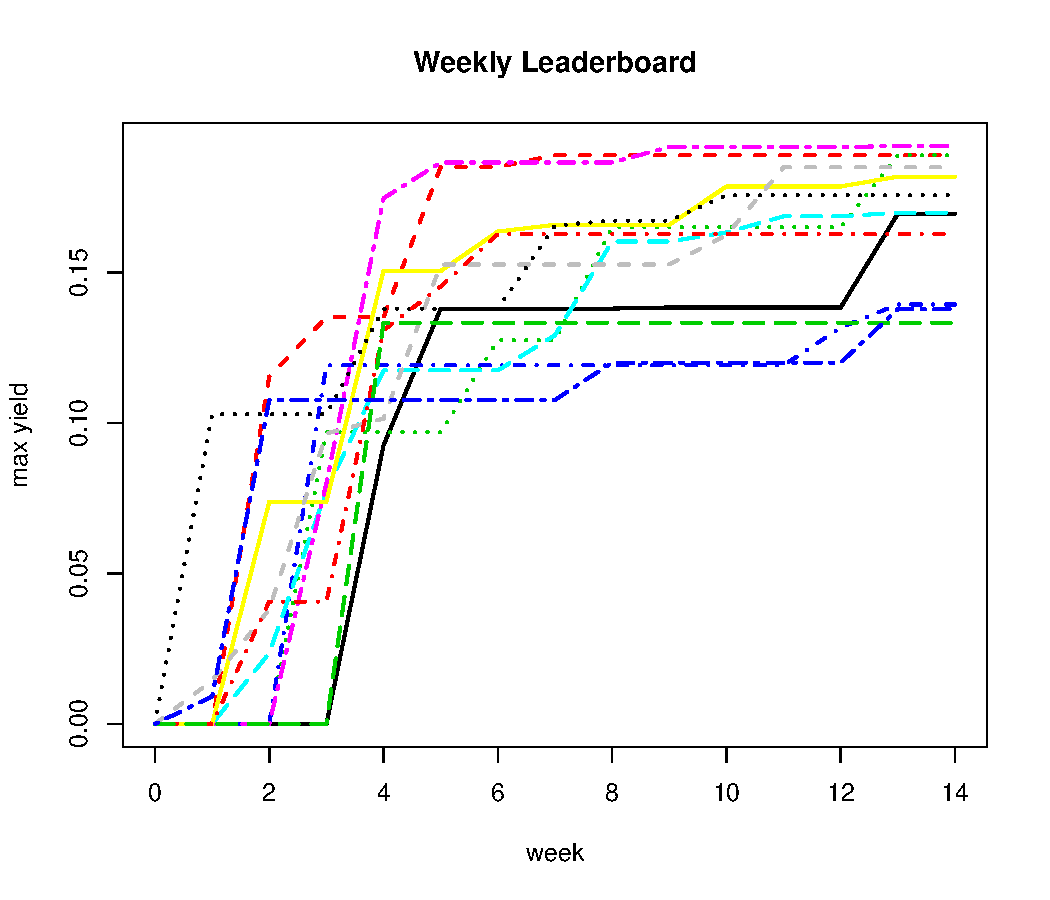
\includegraphics[scale=0.5,trim=0 0 16 0]{weekly_denoised}
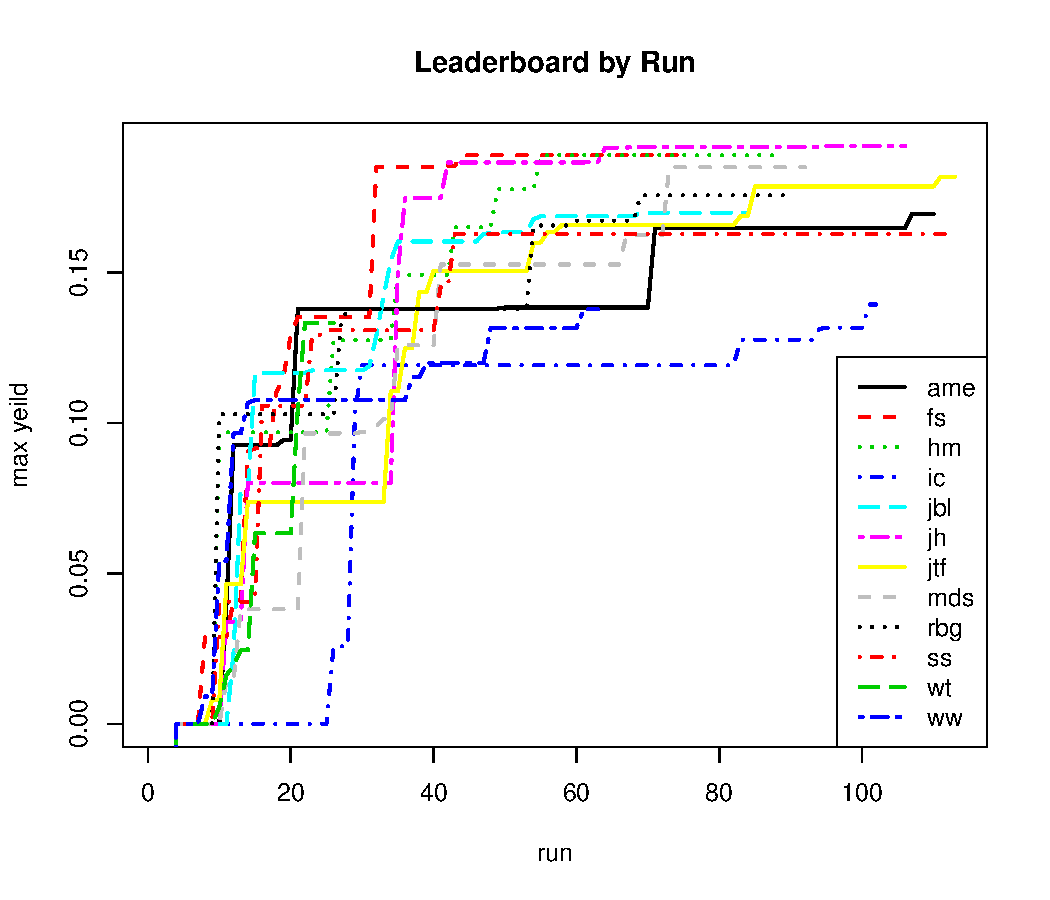
\includegraphics[scale=0.5,trim=50 0 15 0,clip=TRUE]{run_denoised}
\caption{Two de-noised views into the real-time leaderboard during the final
week of game play: best {\tt yield} buy week ({\em left)}, and by run ({\em
right}).}
\label{f:leader}
\end{figure}
Two of those views, snapped during the final week of game play, are provided
in Figure \ref{f:leader}.  On the $x$-axis is the week of game play ({\em
left} panel) or the unique run number ({\em right}), and on the $y$-axis is a
normalized {\tt yield} response value.  Each player has a line in the plot,
with color and type indicated by their initials (masking the pin).  The
responses shown have been de-noised in order to view pure progress, making
normalization essential otherwise players would know the true mean value of
their best noisy response. The two other views provided by the {\tt Rmarkdown}
script show ``raw'' versions of these same plots, on the original
scale---these are not shown here.

Observe from the panel that about half of the progress is made in the first
five weeks, spanning around forty runs.  Students ``jh'' and ``fs'' made rapid
progress.  By contrast, ``hm'' ends up at the same place in the end, but with
more steady increments. The leaderboard would seem to partition students into
three classes, comprising of the top five, middle four, and lower four.
Apparently, students ``wt'' and ``ww'' gave up early.  My own strategy placed
me fifth by these measures.  I favored replication over unique runs in hopes of
obtaining better main effects, sensitivity indices, and estimates of variance
over time.

\section{Discussion}
\label{sec:discuss}

I have described a statistical optimization game updating a previous one in
two senses.  The first sense is that the game uses modern tools for
implementation.  Supplementary materials provide {\sf R} code with support for
a {\tt shiny} app interface, cloud storage for instance-based hosting like
{\tt shinyapps.io}, and real-time views into progress via a leaderboard.
Although the original version of the game was innovative, when introduced it
was essentially unusable by others at the time owing to the nature of
computing environments available in the early 1970s.  The second update has to
do with modern response surface methods.  My re-casting of the game, and the
homework problems from class which support it, emphasize a machine learning
and computer surrogate modeling ``hands-free'' toolkit from the 21st century.

Upon reflection, the game perhaps could be revised to better emphasize these
more modern tools.  Students who made early progress on the leaderboard became
impatient with subsequent lack of positive feedback from further runs.  They
had been ``unlucky'' in finding right answer ``too early'' to benefit from the
modern tools.  In future play I may opt for a multi-modal {\tt yield} surface
in order to keep them engaged, and to demonstrate the explorative value that
comes from EI and IECI-like heuristics appearing later in the syllabus.
Another potentially exciting variation may entertain a real {\tt yield}
simulation, a promising example being the so-called assemble-to-order
\citep[ATO,][]{xie:frazier:chick:2012} solver. This eight-dimensional example is
challenging because it has a spatially dependent noise structure.

\subsubsection*{Acknowledgments}

I am grateful to  students and colleagues at Virginia Tech who helped curate,
and participate in, my class on modern response surfaces and computer
experiments.

\bibliography{yield}
\bibliographystyle{jasa}

\end{document}

Notes:

No ancillary goals revisited at end of paper.  Maybe downplay earlier.

Mention grad class, but could just as well be undergrad.